% --------------------------------------------------------------
%     DENNE MALEN ER LAGET AV MARTIN SORIA RØVANG
%     TIL BRUK FOR OPPGAVELØSNINGER OG RAPPPRTER
%     GITHUB: github.com/martinrovang
% --------------------------------------------------------------


\documentclass[10pt]{article}
\usepackage{amsmath,amsthm,amssymb}
\usepackage{float}
\usepackage[norsk]{babel}
\usepackage[table]{xcolor}
\usepackage{color}
\usepackage{graphicx}
\usepackage{listings}
\usepackage{natbib}
\usepackage[utf8]{inputenc}
\usepackage{imakeidx}
\usepackage[a4paper]{geometry}
\usepackage[myheadings]{fullpage}
\usepackage{fancyhdr}
\usepackage{lastpage}
\usepackage{graphicx, wrapfig, subcaption, setspace, booktabs}
\usepackage[T1]{fontenc}
\usepackage[font=small, labelfont=bf]{caption}
\usepackage{fourier}
\usepackage[protrusion=true, expansion=true]{microtype}
\usepackage{url, lipsum}
\usepackage{tgbonum}
\usepackage{hyperref}
\usepackage{xcolor}
\usepackage[most]{tcolorbox}
\usepackage{mathtools}
\usepackage[page]{totalcount}
\usepackage{lastpage}


\newcommand{\HRule}[1]{\rule{\linewidth}{#1}}
\onehalfspacing
\setcounter{tocdepth}{5}
\setcounter{secnumdepth}{5}
\newcommand{\vect}[1]{\boldsymbol{#1}}

\definecolor{codegreen}{rgb}{0,0.6,0}
\definecolor{codegray}{rgb}{0.5,0.5,0.5}
\definecolor{codepurple}{rgb}{0.58,0,0.82}
%\definecolor{backcolour}{rgb}{0.95,0.95,0.92}
\definecolor{skyblue}{rgb}{0.950, 1, 1}
\definecolor{pink}{rgb}{1, 0.1, 0.5}

\lstdefinestyle{mystyle}{
    backgroundcolor=\color{skyblue},   
    commentstyle=\color{codegreen},
    keywordstyle=\color{magenta},
    numberstyle=\tiny\color{codegray},
    stringstyle=\color{codepurple},
    basicstyle=\footnotesize,
    breakatwhitespace=false,         
    breaklines=true,                 
    captionpos=b,                    
    keepspaces=true,                 
    numbers=left,                    
    numbersep=5pt,                  
    showspaces=false,                
    showstringspaces=false,
    showtabs=false,                  
    tabsize=2,
    frame=single,
    %keywordstyle=\color{blue},
    language=Python
}
 
\lstset{style=mystyle}
\lstset{
    basicstyle=\footnotesize\ttfamily,
  identifierstyle=\bfseries\color{pink!40!pink},
  commentstyle=\itshape\color{black!40!black},
  keywordstyle=\color{blue},
  stringstyle=\color{orange},
}

\newcommand{\N}{\mathbb{N}}
\newcommand{\Z}{\mathbb{Z}}
 
\newenvironment{theorem}[2][Theorem]{\begin{trivlist}
\item[\hskip \labelsep {\bfseries #1}\hskip \labelsep {\bfseries #2.}]}{\end{trivlist}}
\newenvironment{lemma}[2][Lemma]{\begin{trivlist}
\item[\hskip \labelsep {\bfseries #1}\hskip \labelsep {\bfseries #2.}]}{\end{trivlist}}
\newenvironment{exercise}[2][Exercise]{\begin{trivlist}
\item[\hskip \labelsep {\bfseries #1}\hskip \labelsep {\bfseries #2.}]}{\end{trivlist}}
\newenvironment{problem}[2][Problem]{\begin{trivlist}
\item[\hskip \labelsep {\bfseries #1}\hskip \labelsep {\bfseries #2.}]}{\end{trivlist}}
\newenvironment{question}[2][Question]{\begin{trivlist}
\item[\hskip \labelsep {\bfseries #1}\hskip \labelsep {\bfseries #2.}]}{\end{trivlist}}
\newenvironment{corollary}[2][Corollary]{\begin{trivlist}
\item[\hskip \labelsep {\bfseries #1}\hskip \labelsep {\bfseries #2.}]}{\end{trivlist}}

\newenvironment{solution}{\begin{proof}[Solution]}{\end{proof}}
    
\makeindex[columns=3, title=Alphabetical Index, intoc]


% --------------------------------------------------------------
%                         Headers and footers
% --------------------------------------------------------------
\fancyhf{}
\pagestyle{fancy}
\rhead{Martin Soria Røvang}
\lhead{INF-1400-Objektorientert programmering}
\rfoot{Side \thepage \, av \pageref{LastPage}}
\renewcommand{\headrulewidth}{0.3pt}



\begin{document}
% --------------------------------------------------------------
%                         FRONTPAGE
% --------------------------------------------------------------
{\fontfamily{cmr}\selectfont
\title{ \normalsize \textsc{}
		\\ [3.0cm] % How much upper margin
		%\HRule{0.5pt} \\
        \LARGE \textbf{\uppercase{Rapport Oppgave 2}
        \HRule{0.5pt} \\ [0.5cm]
        INF-1400-Objektorientert programmering
        %\HRule{2pt} \\ [0.5cm]
        \\
		\normalsize \today \vspace*{5\baselineskip}}
		}

        \date{}
\author{
		Martin Soria Røvang \\ 
        Universitetet i Tromsø \\}

% \begin{titlepage}
\clearpage\maketitle
\vspace{0.2\textheight}
{\centering
Inneholder \pageref{LastPage} \, sider, inkludert forside.\par
}
\thispagestyle{empty}
% \end{titlepage}

\newpage
\tableofcontents
% --------------------------------------------------------------
%                         Start here
% --------------------------------------------------------------


\newpage

\section{Introduksjon}
I denne oppgaven ble det laget en boid simulator, en simulator som simulerer en flokk. Det beskrives hvordan dette kan bli implementert og hvordan det gjøres med hensyn på objekt-orientert programmering.

\subsection{Krav}


\section{Teknisk bakgrunn}
\emph{Arv(Inheritance)}: Ved å arve fra en annen klasse henter man ut alle egenskapene denne klassen har. Dette kan brukes til å utbedre eller legge til flere ting som er spesialisert, men også bruker andre generelle egenskaper. Dette gjør koden bedre å lese og enklere å bygge på, navigere og feilsøke.[\cite{Dustyphil} p.71\\
\emph{super()}: Super metoden gir deg mulighet til å hente ut metoder eller attributter fra foreldreklassen(parentclass). Hvis du for eksempel skal legge til flere atributter ved instansering av et objekt, men vil også beholde de fra foreldreklassen må man kjøre \emph{super().\_\_init\_\_()} for å hente ut disse [\cite{Dustyphil} p.74].

\section{Design}
\subsection{Klassestruktur}
I dette prosjektet har vi klassestrukturen som vist i figur(\ref{klassestrukturen}) under,
\begin{figure}[hbt!]
{\centering
    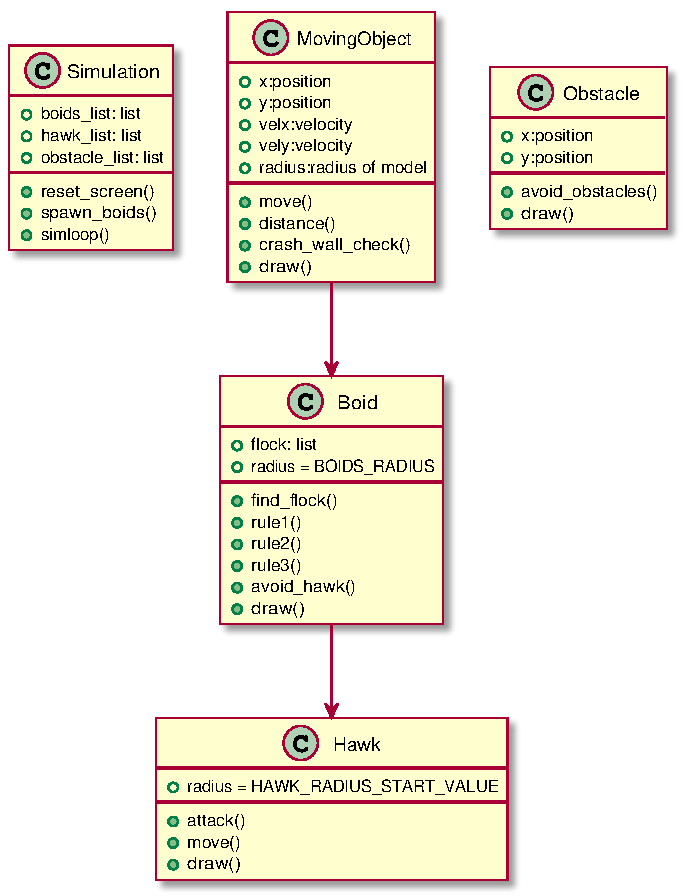
\includegraphics[width=0.50\textwidth]{classes.pdf}
    \caption{Klassestrukturen i programmet.}
    \label{klassestrukturen}
\par}
\end{figure}

Her arver \emph{Boid} klassen fra \emph{MovingObject} og \emph{Hawk}(Hoik) fra Boid. Hvis man arver fra en generell struktur kan man spare kodeplass og generelt får mer strukturert kode. Ved får man også alle metodene og attributtene fra klassen man arver fra[\cite{Dustyphil} p.71]. I noen av klassene ble noen av metodene og attributter erstattet. Dette ble gjort ved å lage en metode som heter det samme i barneklassen(den klassen som arver). Dette gjelder også \emph{\_\_init\_\_()} metoden, derfor vil det oppstå problemer hvis man vil legge inn nye initialattributter, da dette vil erstatte arv-attributtene. et eksempel vil være å gjøre slik som vist i figur(\ref{nye_att}) ved bruk av super()[\cite{Dustyphil} p.74].

\begin{figure}[hbt!]
    \begin{lstlisting}
        class eksempel:
            def __init__(self):
                super().__init__()
                self.a = 10
    \end{lstlisting}
\caption{Lage nye initialattributter og hente de andre fra foreldreklassen}
\label{nye_att}
\end{figure}

\subsection{Simulation}

Simulation er klassen som styrer hva som skal kjøres i programmet. Den har følgene metoder,\\

\begin{itemize}
    \item \emph{reset\_screen}: Fyller skjermen med svart for å overskrive tidligere posisjoner.
    \item \emph{spawn\_boids}: Lager boids hvis man trykker på venstre museknapp.
    \item \emph{simloop}: Dette er den metoden som kjører kontinuerlig i en while-loop så lenge simulasjonsprogrammet er på.
\end{itemize}

\subsection{MovingObject}

MovingObject er en generell funksjon som lager instanser som skal kunne bevege seg, finne distanser til andre bevegelige objekter, unngå å kræsje i vegger og tegne dem.
Dette er en klasse man vil arve fra når man skal ha mer spesifikke klasser som bruker alle/mange av metodene og attributtene til MovingObject.
MovingObject består av funksjonene,

\begin{itemize}
    \item \emph{move}: Beveger objektet etter hvor stor hastigheten er.
    \item \emph{distance}: Returnerer distansen til et annet objekt.
    \item \emph{crash\_wall\_check}: Sjekker om objektet er på vei utafor skjermen. Hvis objektet er på vei ut vil hastigheten bli reflektert og demped. Dette skjer ved å gange hastigheten $\vect{v}$ med en refleksjonskonstant gitt i konfigurasjonefilen.
    \item \emph{draw}: Tegner objektet ut på skjermen.
\end{itemize}

\emph{Move} metoden summer på den tidligere posisjonen og på en enhetsvektor som er skalert av verdi gitt fra konfigurasjonsfilen.

\begin{equation}
    \vect{V} = \frac{\vect{v}}{||\vect{v}||}\alpha
\end{equation}
,der $\alpha$ er en skalar for hva farten skal være slik at,
\begin{equation}
     ||\vect{V}|| = \alpha, \, \forall\,t
\end{equation}

Metoden \emph{distance} finner distansen til et annet objekt ved ta lengden gitt fra pytagoras,

\begin{equation*}
    Distance = \sqrt{(x_{2} - x_{1})^2 + (y_{2} - y_{1})^2}
\end{equation*}

der subindeks $\{1\}$ angir posisjonen til objektet man vil finne lengden fra og $\{2\}$ er posisjonen til objektet man vil finne lengden til.

\subsection{Boid}

Denne klassen inneholder metodene som får objektene til å oppføre seg som en naturlig flokk. Dette blir gjort ved å lage 3 forskjellige regler som kjører kontinuerlig i while-loopen i simulasjons-løkka. Denne klassen arver også fra \emph{MovingObject} derfor vil denne også inneholde alt den også har. Vi har metodene,

\begin{itemize}
    \item \emph{find\_flock}: Putter alle boidsene som tilhører en boid sin flokk i en liste som attributt til en boid. Alle boids vil derfor få en liste med boids(denne tar ikke med boidsen selv).
    \item \emph{rule1}: Finner gjennomsnitts-posisjonen og lager en vektor dit, denne blir summet på hastighetsvektoren til boidsen.
    \item \emph{rule2}: Boidsene unngår å kræsje i hverandre ved å summe på en vektor som er i motsatt retning av boidsen som den er på vei å kræsje med.
    \item \emph{rule3}: Boidsene prøver å matche hastigheten til boidsene som er i sin umiddelbare nærhet.\footnote{Disse reglene ble laget ved bruk av informasjonen på \url{http://www.kfish.org/boids/pseudocode.html}}
    \item \emph{avoid\_hawk}: Summer på vektor som er i motsatt retning av haukene/hoikene slik at de prøver å unngå dem.
    \item \emph{draw}: Tegner dem ut på skjermen.
\end{itemize}

I figur(\ref{rules}) ser man hvordan de tre vektorene kan se ut for en boid.
\begin{figure}[hbt!]
{\centering
    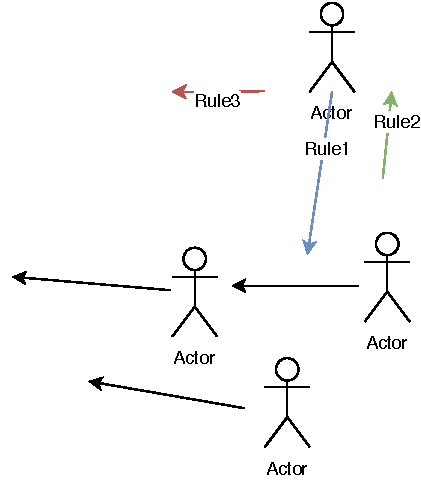
\includegraphics[width=0.30\textwidth]{rules.pdf}
    \caption{De forskjellige vektorene fra regel 1,2 og 3}
    \label{rules}
\par}
\end{figure}

Når disse blir summet opp vil man få en totalvektor som vist i figur(\ref{sumvektor}) under,

\begin{figure}[hbt!]
{\centering
    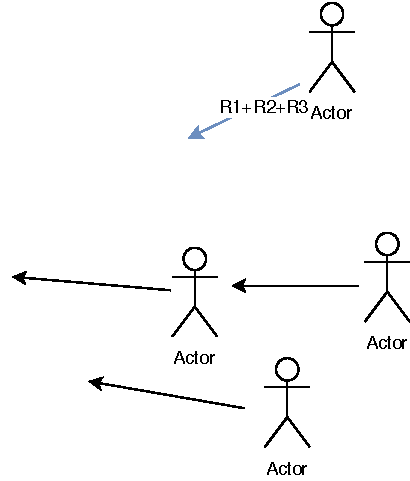
\includegraphics[width=0.35\textwidth]{rulelast.pdf}
    \caption{Summen av vektorene}
    \label{sumvektor}
\par}
\end{figure}

Dette gir en fin og glatt bevegelse til flokkene som ser noe naturlig ut.


\subsection{Hawk/Hoik}

Denne klassen arver fra boids så disse vil oppføre seg likt som dem. Metodene er,

\begin{itemize}
    \item \emph{attack}: Summer opp hastighets-vektoren til hauken som peker i retningen av den nærmeste boiden.
    \item \emph{move}: Lagt til en egen move funksjon fordi hauken har en egen global variabel i konfigurasjonefilen som angir farten uavhengig av boid farten.
    \item \emph{draw}: Tegner hauken/hoiken ut på skjermen.
\end{itemize}


Denne klassen var ganske grei å implementere da det meste var gjort ved arv fra boid klassen.
Noe å ta med seg er at hauken/hoiken bør ha større hastighet enn boidsene, derfor måtte man implementere en ny metode som tok inn egen skalar for hauken.



\subsection{Obstacles}
Dette er en klasse som skal oppføre seg som en vegg for de bevegelige objektene. Metodene er;

\begin{itemize}
    \item \emph{collision}: Sjekker om et bevegelig objekt treffer veggene. returnerer \emph{True} for å bruke det i \emph{avoid\_obstacles} metoden.
    \item \emph{avoid\_obstacles}: Summer opp en hastighetsvektor til boiden/hauken som peker i motsatt retning av veggen slik at de flyr unna. Det er også en test som setter hastigheten til den motsatte retningen om du skulle kræsje med veggen. Distansen fra veggen før boids/hoiks begynner å styre unna er satt i config filen under det globale variabelnavnet \color{purple}{WALL\_DISTANCE\_AVOID\_VALUE}.
\end{itemize}



\section{Implementasjon}
Koden er skrevet i Python versjon 3.7\footnote{https://www.python.org/}\\
OS: Windows 10\\
Systemtype: 64-bit OS, x64-basert prosessor\\
Skjermkort: NVIDIA Geforce 920MX\\
CPU: Intel(R) Core(TM) i5-7200U CPU @ 2.50GHz\\
RAM: 4GB\\
Pygame \footnote{https://www.pygame.org/wiki/GettingStarted} Version: 1.9.4\\
Nympy \footnote{http://www.numpy.org/} Version: 1.14.5\\



\section{Diskusjon}


Via sumulasjons-klassen er det lagt inn mulighet for å lage boids ved å trykke på venstre \emph{musetast}, for hoikene trykker man knappen \emph{C} på tastaturet og for å lage en obstacle trykker man på \emph{A}. Dette ble gjort ved bruk av events i pygame.\footnote{https://www.pygame.org/docs/ref/event.html} 
I denne oppgaven ble pseudokoden fra \url{http://www.kfish.org/boids/pseudocode.html}, dette gjorde det ganske enkelt å implementere reglene for simulatoren. Det vanskligste var å få hoikene/boidsene til å unngå obstacles så fint som mulig og rett og slett angi de riktige størrelsene på skalarene slik at bevegelsene så naturlige ut. Implementasjonen til kantene til simulasjonsvinduet gjorde at det så litt ping-pong ut da boids/hoiks traff dem. Her kunne man ha fjernet veggene ved å for eksempel flytte dem over til den andre siden da de var på vei ut av den ene siden. Dette ville ha skapet litt bedre flyt. Et problem med dette er at de første boidsene/hoiksene som havnet på den andre siden vil miste sine flokk egenskaper da ikke de andre flokk medlemmene har blitt flyttet enda. Dette kan også føre til at hauken/hoiken plutselig vil snu og bevege seg mot den andre siden istedet for å bli med ut av skjermen og også bli flyttet, noe som kan virke unaturlig. Når boidsene kommer nære hindrene(obstacles) så vil de endre retning vekk fra dem. Her brukes senteret av hinderet som referansepunkt for å sjekke avstanden til boidsene. En firkant i pygame har posisjon (x,y) i hjørnet så her må man ta dette med i betraktning når man skal bruke sentrum, slik at $R{sx} = x + width$ og $R{sy} = y + heigth$.


\subsection{Evaluasjon}

Ved bruk av snakeviz\footnote{https://jiffyclub.github.io/snakeviz} kan man visualisere tidsbruk av de forkjellige klassene og metodene. I figur(\ref{Evaluasjon}) ser man en visualisering av dette programmet.

\begin{figure}[hbt!]
{\centering
    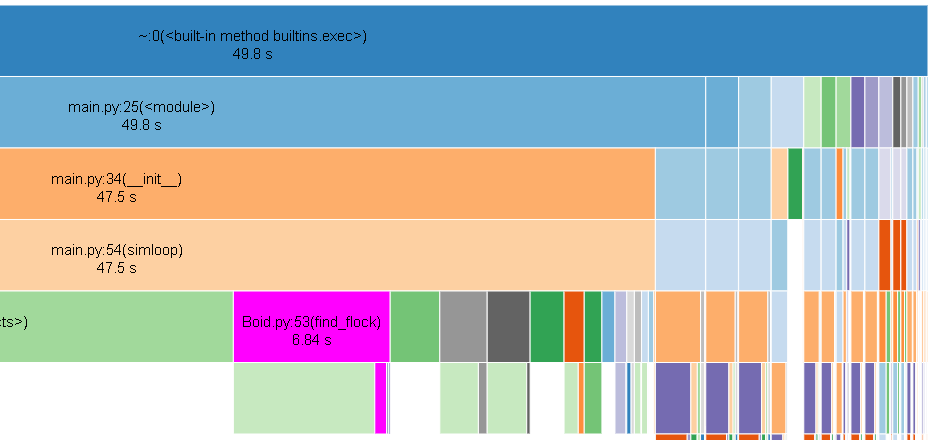
\includegraphics[width=0.70\textwidth]{systeminfo.png}
    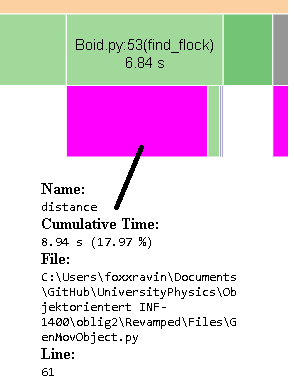
\includegraphics[width=0.50\textwidth]{systeminfo2.png}
    \caption{Visualisering av programmet, her ser man at find\_flock metoden er den som bruker mest tid av de selvskapte metodene, der mesteparten av tidsbruket kommer fra distance metoden.}
    \label{Evaluasjon}
\par}
\end{figure}

Distanse metoden (untatt simloop osv.) er den som bruker mest tid i programmet. Dette er ikke så rart da denne metoden blir kjørt av mange metoder. (rule3, rule2, avoid\_hawk, attack etc). Tar man en titt på find\_flock metoden kan man se en grunn til at dette er den metoden som bruker mest tid. I denne metoden går man igjennom alle boidsene(som kan bli veldig mange) også sjekker man distansen fra en boid til en annen (dette skjer for hver eneste boid!!). deretter blir de lagt inn en liste-attributt som hver boid har.


\section{Konklusjon}

I denne oppgaven så vi på hvordan man kan implementere en boid simulator i python med pygame modulen. Her så man hvordan tre enkle regler gjorde at bevegelige objekter fikk en naturlig flokkbevegelse som man kan observere med blant annet fugler og fisker. Det ble også introdusert rovdyr(hoik) som prøver å spise boidsene for å simulere flokk-rovdyr effekt. Reglene ble implementert ut ifra psuedokoden gitt fra \url{http://www.kfish.org/boids/pseudocode.html}. Det krevde at man finjusterte parametere på hastigheter osv for å få det til å fungere på best mulig måte.





% --------------------------------------------------------------
%     Reference og appendix
% --------------------------------------------------------------
\newpage
\section{Appendix}
\section{Referanser}
\begingroup
\renewcommand{\section}[2]{}%
%\renewcommand{\chapter}[2]{}% for other classes
\bibliographystyle{plainnat}
\bibliography{bibl}
\endgroup



% --------------------------------------------------------------
%     You don't have to mess with anything below this line.
% --------------------------------------------------------------
 





\end{document}

